\documentclass[]{article}

%These tell TeX which packages to use.
\usepackage{array,epsfig}
\usepackage{amsmath}
\usepackage{amsfonts}
\usepackage{amssymb}
\usepackage{amsxtra}
\usepackage{amsthm}
\usepackage{mathrsfs}
\usepackage{color}

%Here I define some theorem styles and shortcut commands for symbols I use often
\theoremstyle{definition}
\newtheorem{defn}{Definition}
\newtheorem{thm}{Theorem}
\newtheorem{cor}{Corollary}
\newtheorem*{rmk}{Remark}
\newtheorem{lem}{Lemma}
\newtheorem*{joke}{Joke}
\newtheorem{ex}{Example}
\newtheorem*{soln}{Solution}
\newtheorem{prop}{Proposition}

\newcommand{\lra}{\longrightarrow}
\newcommand{\ra}{\rightarrow}
\newcommand{\surj}{\twoheadrightarrow}
\newcommand{\graph}{\mathrm{graph}}
\newcommand{\bb}[1]{\mathbb{#1}}
\newcommand{\Z}{\bb{Z}}
\newcommand{\Q}{\bb{Q}}
\newcommand{\R}{\bb{R}}
\newcommand{\C}{\bb{C}}
\newcommand{\N}{\bb{N}}
\newcommand{\M}{\mathbf{M}}
\newcommand{\m}{\mathbf{m}}
\newcommand{\MM}{\mathscr{M}}
\newcommand{\HH}{\mathscr{H}}
\newcommand{\Om}{\Omega}
\newcommand{\Ho}{\in\HH(\Om)}
\newcommand{\bd}{\partial}
\newcommand{\del}{\partial}
\newcommand{\bardel}{\overline\partial}
\newcommand{\textdf}[1]{\textbf{\textsf{#1}}\index{#1}}
\newcommand{\img}{\mathrm{img}}
\newcommand{\ip}[2]{\left\langle{#1},{#2}\right\rangle}
\newcommand{\inter}[1]{\mathrm{int}{#1}}
\newcommand{\exter}[1]{\mathrm{ext}{#1}}
\newcommand{\cl}[1]{\mathrm{cl}{#1}}
\newcommand{\ds}{\displaystyle}
\newcommand{\vol}{\mathrm{vol}}
\newcommand{\cnt}{\mathrm{ct}}
\newcommand{\osc}{\mathrm{osc}}
\newcommand{\LL}{\mathbf{L}}
\newcommand{\UU}{\mathbf{U}}
\newcommand{\support}{\mathrm{support}}
\newcommand{\AND}{\;\wedge\;}
\newcommand{\OR}{\;\vee\;}
\newcommand{\Oset}{\varnothing}
\newcommand{\st}{\ni}
\newcommand{\wh}{\widehat}

%Pagination stuff.
\setlength{\topmargin}{-.3 in}
\setlength{\oddsidemargin}{0in}
\setlength{\evensidemargin}{0in}
\setlength{\textheight}{9.in}
\setlength{\textwidth}{6.5in}
\pagestyle{empty}



\begin{document}


\begin{center}
{\textbf{Experimental modeling of pyroclastic density currents}}\\
Paul A. Jarvis\\ %You should put your name here
\end{center}

\vspace{0.2 cm}

\begin{enumerate}
  %Question 1%%%%%%%%%%%%%%%%%%%%%%%%%%%
\item A simple experiment to model the propagation of a pyroclastic density current (PDC) involves using a configuration as seen in Figure~\ref{fig:flume}. In this setup, there is a gated section which contains the ``gate fluid'' whilst the long section of tank contains the ``environmental fluid''. If the gate fluid density $\rho_{\text{g}}$ is greater than the environmental fluid density $\rho_{\text{e}}$ then, when the barrier between them (gate 2 in Figure~\ref{fig:flume}) is removed the gate fluid will spread along the base of the tank as a gravity current (Figure~\ref{fig:grav_curr}).

  \begin{figure}
    $$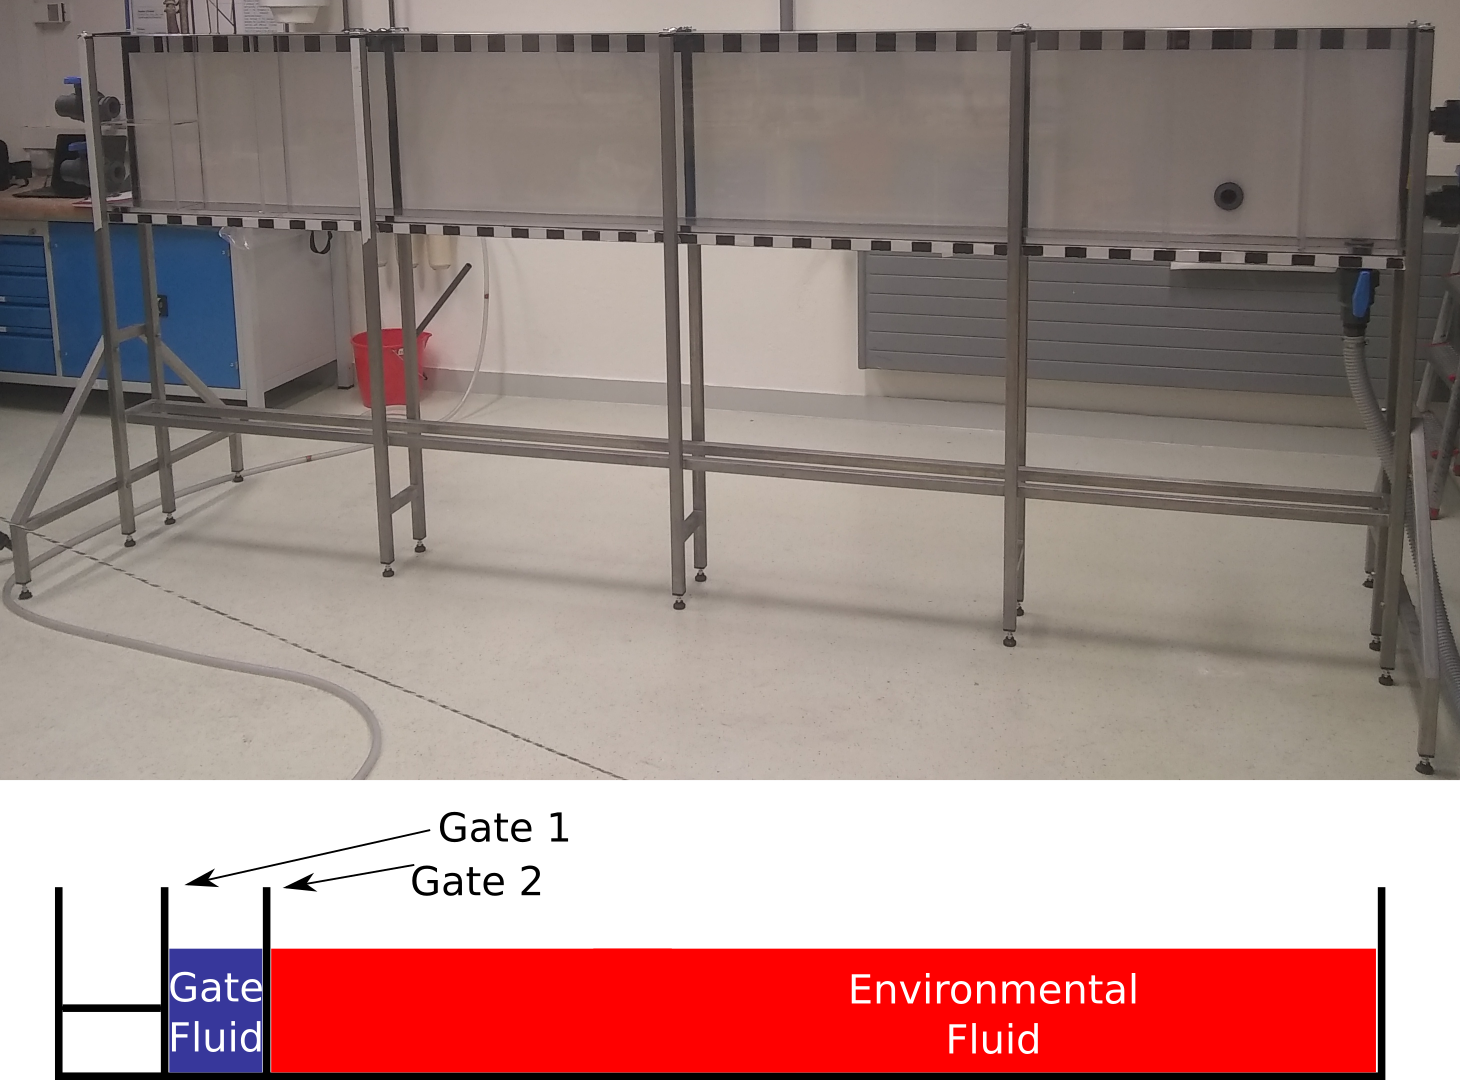
\includegraphics[width=0.75\textwidth]{flume_setup.png}$$
    \caption{The large flume in the Geophysical Fluid Dynamics laboratory. \label{fig:flume}}
  \end{figure}

\begin{figure}
  $$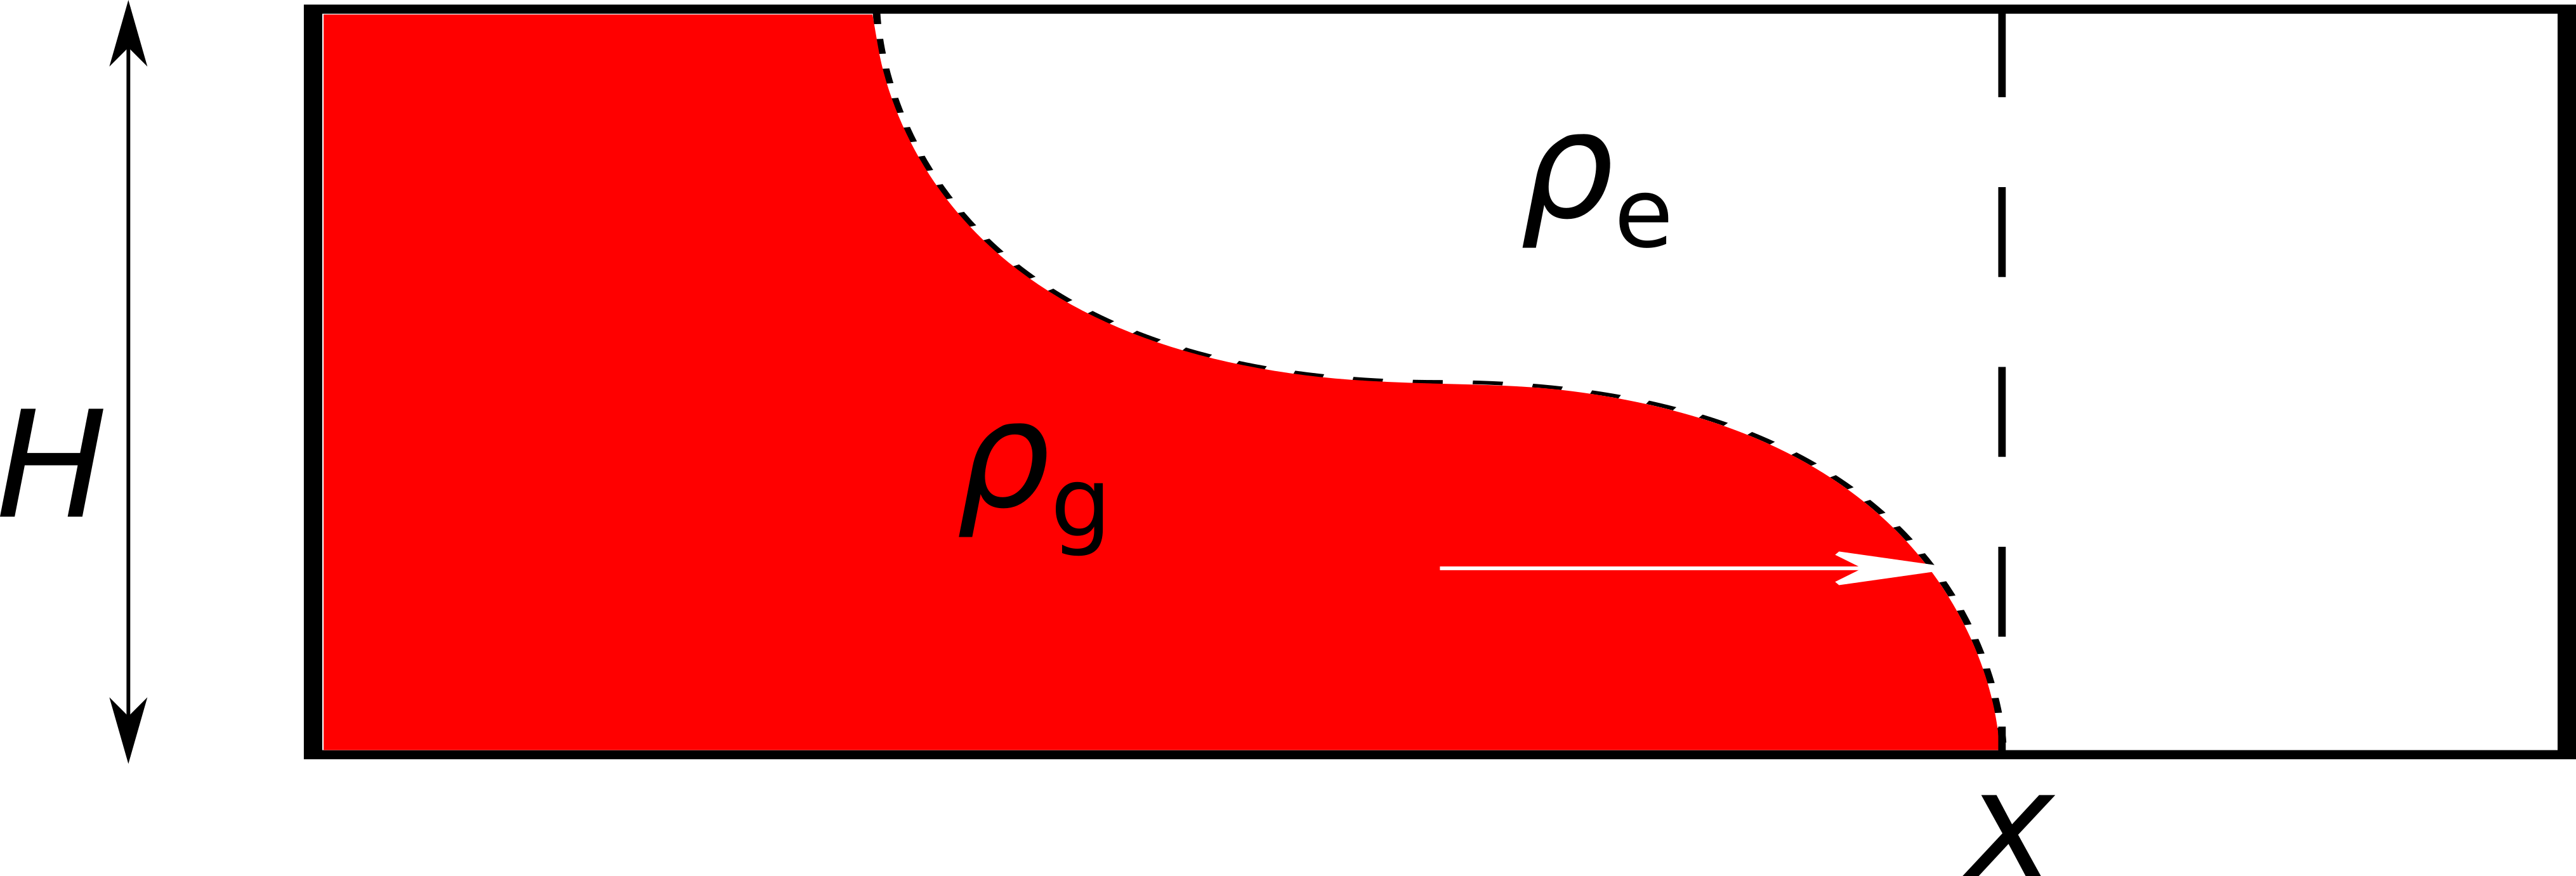
\includegraphics[width=0.75\textwidth]{grav_curr.png}$$
  \caption{Gravity current of density $\rho_{\text{g}}$ propagating in a fluid of depth $H$ and density $\rho_{\text{e}}$. The position of the current head is denoted by $x$. \label{fig:grav_curr}}
\end{figure}

One way to create a density difference between the two fluids is to fill up the whole tank with water before adding the gate. Then, once the gate is in place, dissolve a mass $m_{s}$ of sugar in the gated section to increase the density of the gate fluid. One way to then determine the concentration of the sugar solution is to meausure its refractive index $E_{\text{s}}$ (relative speed of light inside a substance). The sugar concentration $C$ can then be calculated from

\begin{equation}
  \label{equ:equi_sal}
  C = m E_{\text{s}},
\end{equation}

where $m = (12.5 \pm 0.002)$ g l$^{-1}$. Then, the fluid density is calculated by combining $C$ and the temperature $T$ through

\begin{equation}
  \label{equ:dens_model}
  \rho = \rho_{0} [1 + \alpha C+ \kappa (T - T_{0})],
\end{equation}

where $\alpha = (3.87 \pm 0.01) \times 10^{-4}$ l g$^{-1}$ is the solute expansion coefficient, $\kappa = (-2.61 \pm 0.05) \times 10^{-4}$ is the thermal expansion coefficient, $\rho_{0} = (0.99762 \pm 0.00004)$ g l$^{-1}$ and $T_{0} = 293.15$ K.

The attached spreadsheet includes two tables. Table 1 shows the time $t$ at which the head of the current reached fixed positions $x$ in the tank for five different experiments. Tabke 2 contains information showing the mass of sugar added to the gate fluid for each experiment, the refractive indices of the gate and environmental fluids, the temperature and the fluid depth. Note that the environmental fluid often has a non-zero refractive index due to leakage of sugar through the gate.

\begin{enumerate}
\item For each experiment determine the densities of both the gate and environmental fluids, and the reduced gravity $g'$ of the experiment.
\item Produce a figure showung the position of the head of the current $x$ as a function of time $t$ for all experiments.
\item For each experiment, determine the velocity $V$ of the head of the current and then calculate the associated Froude number.
\item Compare each calculated Froude number to that predicted for an ideal gravity current, and give reasons for why they may be different. Think both about what an ideal gravity current means and the limits of the experiment.
\end{enumerate}


When researchers perform laboratory experiments, it is necessary to consider how the results in the laboratory scale to the natural system. If we want to consider how a current in a flume might behave in a larger-scale environment we need to consider the system in a non-dimensional framework. To do this, we need to construct dimensionless position and time variables. 

For the current position $x$, we need to scale $x$ by a lengthscale in the problem. In this case, the appropriate choice is the flow depth $H$. Therefore, the dimensionless current head position is $x' = x / H$.

For the time $t$, we need to find some combination of quantities with units of time. This must be constructed from the parameters involved in the problem: $H$, $\rho_{\text{g}}$, $\rho_{\text{e}}$ and $g$. The suitable combination is $(H / g')^{1/2}$ where $g' = (\rho_{\text{g}} - \rho_{\text{e}}) / \rho_{\text{e}}$ is the reduced gravity. Therefore the dimensionless time is $t' = t (g' / H)^{1/2}$.

\begin{enumerate}\setcounter{enumii}{4}
\item For each experiment, plot $x'$ and a function of $t'$.
\item If the experimental gravity currents where ideal, what would you expect the gradient of $x'(t)$ to be. How does this compare to what you actually see. What could be some reasos for the difference?
\end{enumerate}

Whilst experiments of this nature can be very informative, there will always be details of the natural system which will be neglected.

\begin{enumerate}\setcounter{enumii}{6}
\item Discuss which processes in PDCs are neglected in this simple experimental study and how do you expect them to influence the propagation of the current. Maximum word limit is 500 words.
\end{enumerate}
\end{enumerate}

\end{document}

